\lab{Python}{Computing with Cython}{Cython}
\label{lab:Cython}
\objective{Use Cython when needed to avoid the overhead of some parts of the Python language.
Cython allows for large, time-consuming calculations to be done quickly and near effortlessly in Python.}

For small computations, Python is reasonably fast for computing the solutions to problems.
However, for large computations, Python quickly becomes unable to solve anything in a reasonable amount of time.
You might ask, why use Python at all if it's so slow?
The answer lies in the amount of time to write the code.
Low-level languages like C are renowned for their speed.  These languages are compiled to machine code that can run directly on a computer's processor.
When a C program adds two numbers together, we have to be very specific about what two numbers are added together.
The computer can understand basic data types such as integers, floats, and arrays.
Python represents each of these data types using its own objects.
These are objects are generally fast and we don't notice much the incurred overhead.
Over large calculations, the overhead of these objects is compounded and can slow things down tremendously.
In these cases, we need to be able to access the machine-level data types for integers, floats, and strings for maximum efficiency.
A common way of doing this is to write slower portions of the code in a lower-level, compiled language.
This is usually accomplished by writing a C-extension for Python.
A C-extension is a module that can be used like a Python module, but is written in C.
This enables performance critical code to be executed as fast as possible in a Python environment.
Writing these C-extensions can often be tedious work.

Cython is an optimizing static compiler that accepts both Python and Cython (an extended syntax of Python).
It automates the process of writing a Python C-extension and simplifies to the difficulty of writing Python code.
Cython is a superset of the Python language that enables you to call C functions and declare C types on Python variables.
The additional type declarations of Cython allow it to generate highly optimized C code that will compile with all major C/C++ compilers.
Cython is especially useful for doing large amounts of repetitive calculation, especially when that calculation involves the same data types each time.
Since Cython outputs C code, you can easily call any C function from any point in your Python program.

Cython has a more complex compilation process than Python and is not usually run interactively.
Cython code is usually written in a \texttt{.pyx} file that Cython then translates to a Python C-extension.
The resulting executable is a Python extension that can be imported from the Python interpreter.
Many of the same built in features, data types, and functions from Python work in Cython, but keep in mind that too many calls to Python based functions may slow down a Cython program.
Figure \ref{cython:compilation} shows how a Cython file is compiled and how a function call to a Cython module works.
Regardless of what method you use to compile a Cython file, this is more or less how it works.

\begin{figure}
\centering
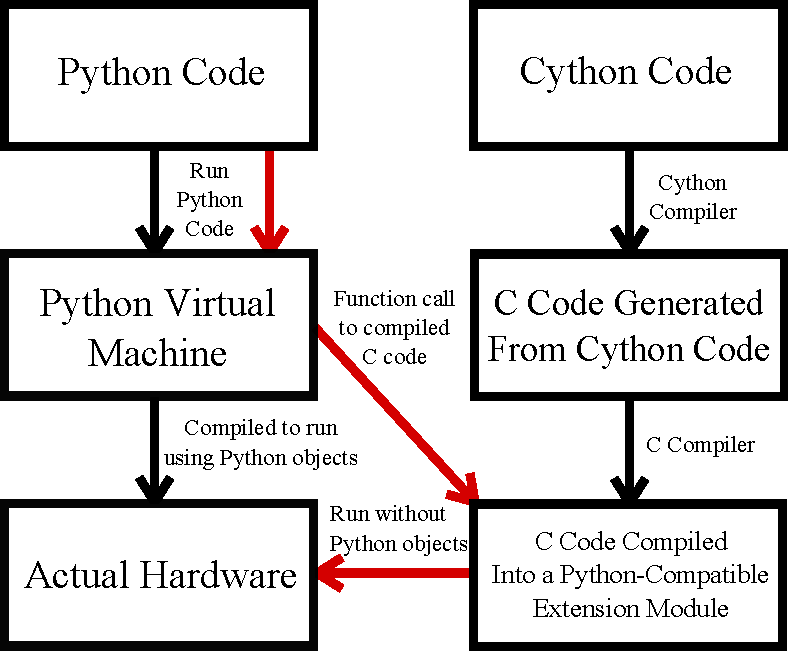
\includegraphics[width=\textwidth]{compilation.pdf}
\caption{A diagram of how Cython compilation and calls to Cython functions work.
The path from using a Cython function in a Python file to the actual evaluation is shown in red.}
\label{cython:compilation}
\end{figure}

There are a variety of ways to import Cython functions and classes into Python.
The standard way is to make a Python file that builds the C-extension module in a given directory.
If your module needs some sort of a complex compilation step, you will need to do it this way.
Instructions on how to do this can be found \url{http://docs.cython.org/src/reference/compilation.html}.
The Sage and IPython notebooks have seamless integrations with Cython via cell magic extensions.
In Sage, the cell magic is \li{\%cython}.
In the IPython notebook, you must first load the extension with \li{\%load_ext cythonmagic}.
Then the first line of any cell containing Cython code should be \li{\%\%cython}.
More instructions on how to use IPython's Cython magic and other related magic functions can be found in the IPython documentation.
Cython also comes with a Python module, \li{pyximport}, that will automatically generate, compile, and import most Cython files.
\begin{lstlisting}
import pyximport
pyximport.install()
\end{lstlisting}

\section*{Type Declarations}
One of the easiest ways improve performance in Cython is declaring types on variables.
While it is good practice to try and restrict variables to a single type (doing so can improve performance in Python program),
Python does not enforce strict type checking.  In fact, Python variables are dynamically typed.  
Any variable can be any type and that type can change at any time.
To allow this behavior, lots of background checking must be performed.
Cython allows us to declare a variable of a certain type.  If we declare a variable an integer, then an integer it will be for the remainder of its life.
These typed variables are not Python objects, but native machine-types.
In Python, you can iterate over a list, or use a generator object.
In C, for-loops are managed by indexing an integer and checking to see if it is within a range of allowed values.
This is a good example of a time when Python objects can incur significant overhead.
In Python to do a for-loop from 0 to 1000000 you would do something like this:
Doing a for-loop in this way creates a Python list of 1000000 objects and then iterates through it.
This can  be very slow.
\begin{lstlisting}
for i in range(1000000):
    pass
\end{lstlisting}
It also uses a great deal of memory for no particular reason
We can improve on this by using the \li{xrange} function as follows:
\begin{lstlisting}
for i in xrange(1000000):
    pass
\end{lstlisting}
This skips making the list and makes a generator object which returns the values as we need them.
For large lists, this can give us a speedup of a factor of 3 or 4 times.
Because of this, the \li{range} function in Python 3 was changed to behave as the \li{xrange} function of Python 2.
However, \li{xrange} still generates a sequence of Python integers.
Cython will also execute this loop in the Python interpreter.
But, we can give Cython a little hint as to how to speed up the loop by telling it the type of the variable \li{i}.
If we do this, we can completely relieve the Python interpreter of executing the loop.
We use a \li{cdef} statement to define \li{i} as a C integer type with this syntax \li{cdef <type> <name>}.
The empty for-loops above would be written in Cython as follows:
\begin{lstlisting}
cdef int i
for i in range(1000000):
    pass
\end{lstlisting}
Because Cython has the extra type information regarding the loop, it can translate the loop into C which is roughly 50 times faster than using the generator in Python.
Cython is able to do this by removing the overhead of working with Python integer objects.
Similar ideas also apply to repeated operations with other types of variables.
For example, if you have an array of double precision floating point values and you want to take the sum of all of them, your code will run faster if you declare the types of all the variables you use before you do any computation.
It is much easier for your computer to perform arithmetic operations without having to infer what datatypes are being used, what types need to be modified before computation can actually be done, and which version of each operation needs to be performed.
Adding types unnecessarily may not actually result in an increase in performance. If it is done poorly it can actually slow things down, but if you have a large number of computations involving the same data type, adding type declarations should speed things up considerably.
Statements using \li{cdef} are also not allowed inside loops, so you will have to declare all the variables you need before you use them.

\section*{Optimized Array Access}
Often, we want to iterate over large arrays very quickly.
In Python, the \li{__getitem__} method (i.e. array access using \li{[ ]}) of NumPy arrays is written for Python and includes the corresponding overhead.
As before, we would like to get around the extra cost involved with Python objects.
There are several ways this can be done.
If the array is an intermediate array in the program, it could possibly be replaced entirely with a C array in Cython, but this may not interface nicely with Python code for returning values, etc., so we would like to avoid that option.
Fortunately, Cython includes a direct interface to part of NumPy.
NumPy arrays are already implemented in C, so we can use this interface to work directly with NumPy arrays.
A typed NumPy array can be declared like this:
\begin{lstlisting}
cimport numpy as np
...
cdef np.ndarray[dtype=double, ndim=2] X = ...
\end{lstlisting}
You can also use an additional argument, \li{mode}, to specify if the array is to be C-contiguous, Fortran-contiguous, full, or strided (\li{c}, \li{fortran}, \li{full}, and \li{strided} respectively).
An array is said to be C contiguous when neighboring values of the last dimension are closest together in memory.
Fortran-contiguous arrays store data in the opposite ordering with neighboring values in the first dimension closest together.
For a 2D array, C-contiguous ordering puts rows in continuous blocks of memory while Fortran-contiguous stores by column.
The syntax to declare arrays like this is:
\begin{lstlisting}
cimport numpy as np
...
#C-contiguous
cdef np.ndarray[dtype=double, ndim=2, mode=`c'] X = ...
\end{lstlisting}
Declaring our arrays like this allows us to access individual items in a NumPy array at roughly the same speed we could access items in a C array.
We get all the convenience of using a NumPy array and can still use the different array operations, but we also get to access single items in the array more quickly.
The catch is that this fast array access only works when we are accessing the array \textit{one item at a time}.
Generally we can get around the slicing, but if we need to pass around NumPy array slices between the functions in the module, there can be a significant speed loss (these array slices are Python objects).
Cython has a \li{memoryview} object designed for this.
Memoryviews support the same fast indexing as the NumPy arrays and slices of memoryviews continue to support the optimized buffer access.
%% I'll demostrate this in the solutions
They are useful when you need to pass array slices between functions in your module.
They also work especially well when used in inline functions, and the corresponding syntax is relatively simple.
%%will demonstrate benefits of inlining as well
However, passing a memoryview object to a NumPy function becomes slower as the memoryview has to be converted to a NumPy array.
%%also shown in solutions
If you need to use NumPy array functions and pass memory views between functions you can define a \li{memoryview} object that views the same data as your array.
If for some reason you need to convert a memory view to a NumPy array, you can use the \li{np.asarray} function, but that, as always, comes at a cost.
The syntax to use when declaring a memory view of an array \li{X} is:
\begin{lstlisting}
cdef double[:,:] Xview = X
\end{lstlisting}
If we know more about the memory layout of \li{X} we can also add that to the type declaration.
Knowing that \li{X} is C-contiguous (which is normally true for a newly initialized NumPy array) the following works:
\begin{lstlisting}
cdef double[:,::1] Xview = X
\end{lstlisting}
When the array is Fortran-contiguous we can use the following:
\begin{lstlisting}
cdef double[::1,:] Xview = X
\end{lstlisting}

It is also worth noting that many of the array operations in Cython can also be done using pointers.
The speed is roughly the same as with the optimized array lookups, but the code is often much less readable.
Cython does not allow you to dereference a pointer using the \li{*} syntax.
You should use square brackets \li{[ ]}.

\section*{Compiler Directives}
There are also some compiler directives you can pass to the Cython compiler which will speed up array access.
By default, Cython checks to see if the indices used in array accesses are within the bounds of the array.
Cython also allows negative indexing the same way Python does.
These features incur some performance loss and may be removed once a program has been carefully debugged.
Compiler directives in Cython can be included as comments or as function decorators.
Directives included in comments will apply to the whole file, while function decorators will only apply to the function or method immediately following the decorators.
The comments to turn off bounds checking and negative indices are, respectively:
\begin{lstlisting}
#cython: boundscheck=False
#cython: wraparound=False
\end{lstlisting}
To use the function decorators you must first include the \li{cython} module.
This is done by including the line \li{cimport cython} in your import statements.
The decorators are:
\begin{lstlisting}
cimport cython
@cython.boundscheck(False)
@cython.wraparound(False)
\end{lstlisting}
When using these compiler directives, you must be \emph{absolutely certain} that you are \emph{not} using negative indices or accessing any array out of bounds.
Doing so could access and possibly modify some portion of memory that has not been allocated as part of an array.
That can cause all kinds of trouble.
It is usually best to only include these directives after you have finished debugging your program.

Cython has several other useful compiler directives.
One that you should be aware of is the \li{cdivision} option.
In Python, the \li{\%} operator returns a number with the sign of the second argument, while C keeps the sign of the first argument.
In Python, \li{-1\%5} returns \li{4}, while in C, this returns \li{-1}.
Cython, by default, will behave like Python.
Cython will also check for zero division and raise a \li{ZeroDivisionError} when necessary.
Again, this does cost a little, so if you are working with integer division and want a slight speedup, you can set \li{cdivision} to \li{True} in the same way you would change the \li{boundscheck} and \li{wraparound} options.
This will make the \li{\%} operator behave like it would in C and turn off the check for zero division.

\section*{Functions in Cython}
As you may expect, adding type declarations can also apply to function arguments in Cython.
You can optionally declare the types of the inputs for the function to ensure that it receives the right arguments.
The syntax is what you would probably expect.
\begin{lstlisting}
def myfunction(np.ndarray[dtype=double, ndim=1] X, int n, double h, items):
    ...
\end{lstlisting}
Notice that we did not have to include type declarations for all of the arguments.
The untyped arguments are expected to be Python objects with the corresponding methods.
Computations involving these untyped arguments will use Python instead of C.
Keyword arguments are also supported.

Cython also allows you to make C functions that are only callable within the extension library you are currently building.
The type declarations for these functions are a little more useful (you don't usually gain much by declaring a type for a Python function).
These functions are declared using the same syntax as you would in Python except that you replace the keyword \li{def} with \li{cdef}.
These functions can be called within the module you are building, but are not actually imported into your namespace when you load the Cython module.

Cython also allows you to declare functions using the \li{cpdef} statement.
These functions are C functions that, when compiled, are also wrapped as Python functions so they can be called in Python.
This allows you to do the function calls within the module in C, while still making a Python wrapper for your function available for use outside the module itself.
You can specify the return type for functions declared using \li{cdef} and \li{cpdef} like you would a variable, for example:
\begin{lstlisting}
cpdef int myfunction(np.ndarray[dtype=double, ndim=1] X, int n, double h, items):
    ...
\end{lstlisting}
This will make two functions, one will be a C function which will return an integer value.
The other will be a Python wrapper for the C function.
The Python-accessible function will accept all the same arguments and return the same value, but it will be callable from Python.

\section*{Some Examples}
To illustrate how to use Cython we will take the dot product of two one-dimensional arrays.
This would be done in Python like this:
\begin{lstlisting}
def pydot(A, B):
    tot = 0.
    for i in xrange(A.size):
        tot += A[i] * b[i]
    return tot
\end{lstlisting}
Assuming we are using the IPython notebook we can define and compile a cython function to do this by evaluating the following cells:

\begin{lstlisting}
%load_ext cythonmagic
\end{lstlisting}

\begin{lstlisting}
%%cython
from numpy cimport ndarray as ar
cimport cython

@cython.boundscheck(False)
@cython.wraparound(False)
def cydot(ar[double] A, ar[double] B):
    cdef double tot=0.
    cdef int i
    for i in xrange(A.size):
        tot += A[i] * B[i]
    return tot
\end{listlisting}
We can then time our function by evaluating the following cell
\begin{lstlisting}
from numpy.random import rand
n = 10000000
A = rand(n)
B = rand(n)
%timeit cydot(A, B)
\end{lstlisting}

Figure \ref{cython:dot} compares the timings of our new dot-product function with other possible implementations.

\begin{figure}
\centering
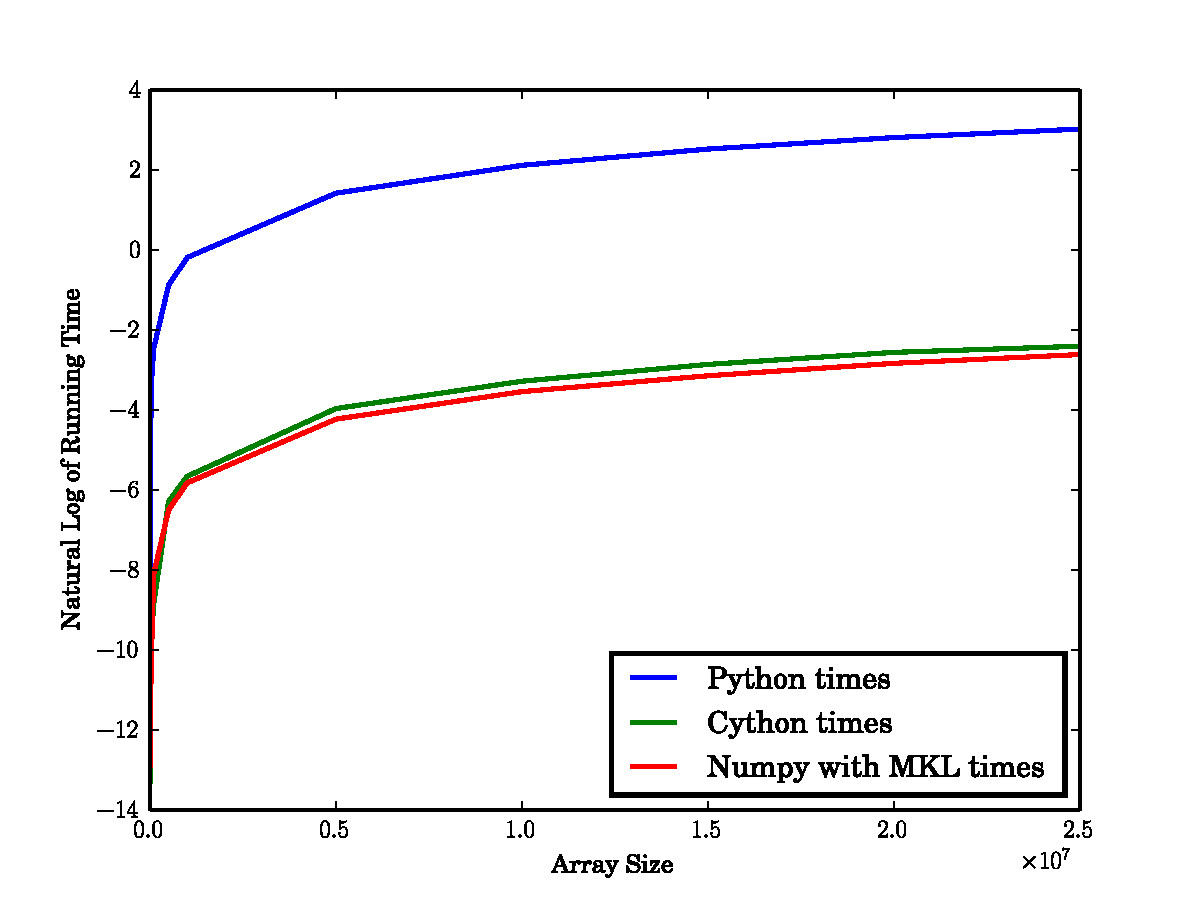
\includegraphics[width=\textwidth]{dot.pdf}
\caption{
The natural logarithm of the times of the pure Python dot-product, the Cython based dot-product, and the dot-product built into NumPy which links to the Intel MKL.
As you can see, the Cython version can run nearly as fast as the version built into NumPy.
}
\label{cython:dot}
\end{figure}

Now we will do a more advanced example using memoryviews.
We will write functions which, given a two-dimensional array \li{A}, make a new array \li{B} for which, \li{B[i,j] = dot(A[i],A[j])}.

Here's a purely iteration-based solution in Python.
\begin{lstlisting}
def pyrowdot(A):
    B = np.empty((A.shape[0], A.shape[0]))
    for i in xrange(A.shape[0]):
        for j in xrange(i):
            temp = pydot(A[i], A[j])
            B[i,j] = temp
        B[i,i] = pydot(A[i],A[i])
    for i in xrange(A.shape[0]):
        for j in xrange(i+1,A.shape[0]):
            B[i,j] = B[j,i]
    return B
\end{lstlisting}

To do this same sort of thing in Cython we can compile the following file:

\begin{lstlisting}
import numpy as np
from numpy cimport ndarray as ar
cimport cython

@cython.boundscheck(False)
@cython.wraparound(False)
cpdef inline cydot(double[:] A, double[:] B, int n):
    cdef double tot=0.
    cdef int i
    for i in xrange(n):
        tot += A[i] * B[i]
    return tot

@cython.boundscheck(False)
@cython.wraparound(False)
def cyrowdot(ar[double, ndim=2] A):
    cdef ar[double, ndim=2] B = np.empty((A.shape[0], A.shape[0]))
    cdef double[:,:] Aview = A
    cdef double temp
    cdef int i, j, n=A.shape[0]
    for i in xrange(n):
        for j in xrange(i):
            temp = cydot(Aview[i], Aview[j], n)
            B[i,j] = temp
        B[i,i] = cydot(Aview[i], Aview[i], n)
    for i in xrange(n):
        for j in xrange(i+1,n):
            B[i,j] = B[j,i]
    return B
\end{lstlisting}

This can also be done in NumPy by running \li{A.dot(A.T)}.
The timings of the Python and Cython versions of this function are shown in Figure \ref{cython:rowdot}.

\begin{figure}
\centering
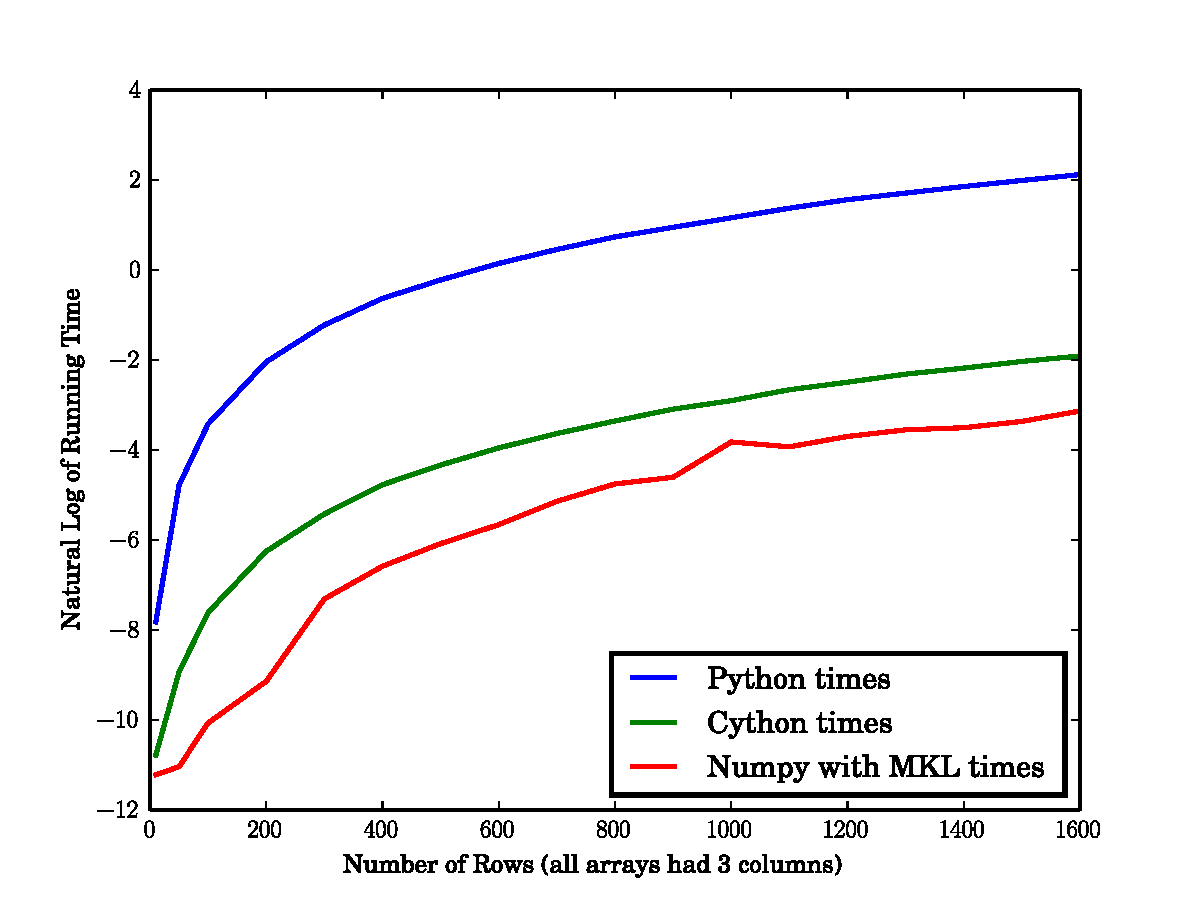
\includegraphics[width=\textwidth]{rowdot.pdf}
\caption{
The natural logarithms of the times of the Python, Cython, and NumPy (with MKL) versions of the \li{rowdot} function that we used as an example.
The arrays used for testing were $n\times 3$ where $n$ is shown along the horizontal axis.
}
\label{cython:rowdot}
\end{figure}

\begin{problem}
Write a function in Python which takes the sum of a one-dimensional array by iterating over it.

Write three Cython versions also, one which uses a typed for-loop to iterate over the array, one which uses a typed for-loop and optimized array access, and one which uses a typed for-loop, optimized array access, and special compiler directives to further speed up array access

Compare the speed of the functions you just wrote, the builtin \li{sum()} function and NumPy's \li{sum()} function.
What do you see?
Notice that when you type your variables in ways that don't work well, you may actually slow things down.
\end{problem}

\section*{Using C Functions and Data Types in Cython}
Cython also allows you to easily interface between Python and C.
It comes with many of the basic math functions from the math library already implemented.
These functions can be imported using something along the lines of:
\begin{lstlisting}
from libc.math cimport fabs, sin, cos, ...
\end{lstlisting}
Notice that we imported \li{fabs}.
This is the absolute value function from C, but it is imported as fabs so that it does not overwrite Python's built in \li{abs} function. 
\li{min} and \li{max} are also renamed the same way.
These functions are good for large amounts of computation when we don't want to deal with the overhead from Python objects.
Cython also allows you to import other C functions and libraries.
It can make wrapping these libraries much easier.

\begin{problem}
In an earlier lab, you wrote a function to compute the LU decomposition of nonsingular matrix.
Port it to Cython.
Use the typed for-loops, typed arrays (or memory views), and the additional compiler directives in your optimized solution.
You may assume, in this case, that you are only dealing with real arrays of double precision floating point numbers.

Compare the speed of your new solution to the speed of the Python based version you wrote earlier.
For testing the speed of your solutions, you can generate large, symmetric, positive-definite arrays by first generating a random array of floating point values, then multiplying it by its transpose (here we mean matrix multiplication using \li{np.dot()}).
\end{problem}

\begin{problem}
The code below defines a Python function which takes a matrix to the $n$th power.
Port it to Cython. Write three different versions: one which use typed arrays, another using typed arrays with the special compiler directives, and another using typed arrays with corresponding typed memory views of their corresponding data and the compiler directives.
\begin{lstlisting}
import numpy as np
def mymult(X, power):
    prod = np.empty_like(X)
    prod[:] = X
    temparr = np.empty_like(X[0])
    size = X.shape[0]
    for n in xrange(1, power):
        for i in xrange(size):
            for j in xrange(size):
                tot = 0.
                for k in xrange(size):
                    tot += prod[i,k] * X[k,j]
                temparr[j] = tot
            prod[i] = temparr
    return prod
\end{lstlisting}

Compare the speed of the Python function, the three functions you just wrote, and the \li{np.dot()} function.
The NumPy function should be faster, but only by an order of magnitude or so.
NumPy and SciPy do this computation and other computations by calling BLAS and LAPACK, very optimized Fortran libraries for linear algebra.
This is probably one of the best-optimized portions of NumPy and Scipy.
The difference in performance should be particularly clear in this case because of the high order of complexity of the algorithm.
\end{problem}

It is important to recognize that the choice of algorithm and fast implementation can both drastically affect the speed of your code.
A simple example is the tridiagonal algorithm (also called the Thomas Algorithm) which is used to solve systems of the form:
\[
\begin{bmatrix}
b_0 & c_0 & 0 & 0 & 0 & \cdots & \cdots & 0 \\
a_0 & b_1 & c_1 & 0 & 0 & \cdots & \cdots & 0 \\
0 & a_1 & b_2 & c_2 & 0 & \cdots & \cdots & 0 \\
0 & 0 & a_2 & b_3 & c_3 & \cdots & \cdots & 0 \\
\vdots & \vdots & \vdots & \vdots & \vdots & \ddots & \ddots & \vdots \\
\vdots & \vdots & \vdots & \vdots & \vdots & \ddots & \ddots & c_{n-1} \\
0 & 0 & 0 & 0 & 0 & \cdots & a_{n-1} & b_n 
\end{bmatrix}
\begin{bmatrix}
d_0\\
d_1\\
d_2\\
d_3\\
\vdots\\
\vdots\\
d_n
\end{bmatrix}
=
\begin{bmatrix}
x_0\\
x_1\\
x_2\\
x_3\\
\vdots\\
\vdots\\
x_n
\end{bmatrix}
\]
The following Python code solves this system.
Notice that \li{x} and \li{c} are modified in place.
The final result is stored in \li{x}, and \li{c} is used to store temporary values.
\begin{lstlisting}
def tridiag(a, b, c, x):
    #note: overrides c and x
    size = x.size
    temp = 0.
    c[0] = c[0] / b[0]
    x[0] = x[0] / b[0]
    for n in range(size-2):
        temp = 1. / (b[n+1] - a[n]*c[n])
        c[n+1] *= temp
        x[n+1] = (x[n+1] - a[n]*x[n]) * temp
    x[size-1] = (x[size-1] - a[size-2]*x[size-2]) / (b[size-1] - a[size-2]*c[size-2])
    for n in range(b.size-2, -1, -1):
        x[n] = x[n] - c[n] * x[n+1]
\end{lstlisting}

\begin{problem}
Port the above code to Cython using typed for loops, optimized array accesses and the special compiler directives.
Compare the speed of your new function with the pure Python version given above.
Now compare the speed of both of these functions with the \li{solve()} function in \li{scipy.linalg}.
For your first two functions a good starting point for computation will be to consider $1000000 \times 1000000$ sized systems and then adjust the size so you get good results on your particular machine.
When testing the SciPy algorithm, you will probably want to start with systems involving a $1000 \times 1000$ matrix and then go up from there.
Keep in mind that the SciPy function is heavily optimized, but that it uses a much more general algorithm.
What does this example tell you about the relationship between good implementation and proper choice of algorithm?
In this case, the LU decomposition method used by the SciPy function has complexity $O(n^3)$, while the tridiagonal algorithm is $O(n)$.
\end{problem}
